\documentclass[11pt, english]{article}              
        \usepackage{geometry}
                \geometry{                          
                        a4paper,total={210mm,297mm},
                        tmargin=40.8mm,
                        bmargin=40.8mm,
                        lmargin=32.6mm,        
                        rmargin=32.6mm,                     
                }                                     
                                
        \usepackage{titlesec}         
                \titleformat{\section}
                        {\normalfont\fontsize{18}{16}\bfseries}{\thesection}{0.5em}{}
                \titleformat{\subsection}
                        {\normalfont\fontsize{14}{16}\bfseries}{\thesubsection}{1em}{}
                \titleformat{\subsubsection} 
                        {\normalfont\fontsize{11}{16}\bfseries}{\thesubsubsection}{1em}{}
                                                                    
        \usepackage{longtable}                                                  
        \usepackage{multirow}                                                   
                             
        \usepackage[labelfont=bf,textfont=bf,font=small,skip=8pt]{caption}
                               
        \setlength{\parindent}{0pt}                                 
        \renewcommand{\baselinestretch}{1.25}      
        \usepackage{setspace}                             
                                                                        
        \usepackage{amsmath}                                                    
        \usepackage{amssymb}                                      
                             
        \usepackage{graphicx}                  
                               
        \usepackage{float}                                                
                                                  
\begin{document}                               
                                              
\pagenumbering{gobble}       
                       
        \title{\textsc{EC315 Topics in Microeconomics with Cross-Section Econometrics\\ Coursework Summary}}
        \author{\textsc{Lewis Britton}}
        \date{\textsc{Academic Year 2019/2020}}
        \maketitle
                                                                                                                                 
\newpage
                         
\pagenumbering{roman} 
                                                                           
        \renewcommand{\contentsname}{Table of Contents}
                                       
        \tableofcontents

\newpage 

\pagenumbering{arabic}

\section{Exam Summary}

	\subsection{Cost-Benefit Analysis Summary}

	\begin{enumerate}
	\setlength\itemsep{0cm}
		\item Purpose
		\item Alternatives
		\item Who
		\item C/B Impacts
		\item Lifetime Impacts
		\item Monetize:
		\begin{itemize}
			\item \textit{Social Cost}: harm done to living organisms
			\item \textit{Revealed/Stated Preference}: willingness to pay or willingness to accept
			\begin{itemize}
				\item Revealed: shown in behaviour
				\item Stated: questionnaires etc.
			\end{itemize}
			\item \textit{Time}:
			\begin{itemize}
				\item Work vs leisure using wage rate 
				\item Travel time; how much people are willing to trade-off
			\end{itemize}
			\item \textit{Lives}: life expectancy, pay, age, risks taken
			\item \textit{Natural Resources}: AONBs, surveys, investment, regulation
		\end{itemize}
		\item PV Discounts
		\begin{itemize}
			\item Social discount rate
			\item Intergenerational (more than 50 years)
		\end{itemize}
		\item NPV of Alternatives
		\item Sensitivity Analysis
		\item Recommend
	\end{enumerate}

	\newpage

	\subsection{Program \& Policy Evaluation Summary}

	\begin{center}Cause $\longrightarrow$ Intermediaries $\longrightarrow$ Effect\end{center}

	\begin{enumerate}
	\setlength\itemsep{0cm}
		\item Omitted Variable Bias
		\begin{itemize}
			\item Selection Bias: e.g. grades, income, area of ogigin
			\item Selection Bias 2: e.g. effort, determination, stamina
		\end{itemize}
		\item Randomized Control Trial
		\begin{itemize}
			\item Unbiased Estimator: $\bar{x}\longrightarrow\bar{\mu}$ (LLN)
			\item Unbiased Estimator: randomization
			\item $\sigma^2$: ``how much of the result is due to chance?''
			\item t-tests: causal effect; $(\bar{Y}^T-\bar{Y}^C)$
		\end{itemize}
		\item Regression
		\begin{itemize}
			\item Dummy Variables: causal variable / group
			\item Instrumental Variables: omitted variables ($\alpha$ corr. w/ $\varepsilon$)
		\end{itemize}
	\end{enumerate}

	\newpage

	\subsection{Crime \& Punishment Summary}

	\begin{enumerate}
	\setlength\itemsep{0cm}
		\item Supply: $\pi_t=\pi_i-c_i-w_i-p_i(f_i)$
		\begin{itemize}
			\item $i$ = Individual
			\item $\pi_t$ = Net Total Payoff of Crime
			\item $\pi_i$ = Expected Payoff Per Offense (Minus Costs)
			\item $c_i$ = Cost Incurred if Caught
			\item $w_i$ = Wage Rate From Non-Criminal Work
			\item $p_i$ = Probability of Aprehension \& Conviction
			\item $f_i$ = Punishment in Convicted
		\end{itemize}
		\item Normal Distribution
		\begin{itemize}
			\item Req. $\uparrow\pi,\ \uparrow\delta,\ [\bar{x}\rightarrow\mathrm{(Right\ of\ Mean)}]$
			\item Req. $\downarrow\pi,\ \downarrow\delta,\ [\leftarrow\bar{x}\mathrm{(Left\ of\ Mean)}]$
			\item Morals, enjoyment, risk, some demand for significantly higher payoffs etc. effect decision
		\end{itemize}
		\item Demand: $e_if(v_r,v_l);q$
		\begin{itemize}
			\item $e_i$ = Expenditure on Protection
			\item $v_r$ = Risk of Victimization
			\item $v_l$ = Loss of Victim
			\item $q$ = Total Crime
		\end{itemize}
		\item Derivatives
		\begin{itemize}
			\item $\frac{\partial e_i}{\partial v_i}>0$: Risk $\uparrow$, Expenditure $\uparrow$
			\item $\frac{\partial c_i}{\partial e_i}<0$: Expenditure $\uparrow$, Cost $\uparrow$
			\item $\frac{\partial\pi_i}{\partial c_i}<0$: Cost $\uparrow$, Payoff $\downarrow$
		\end{itemize}
		\item Supply / Demand
		\begin{itemize}
			\item 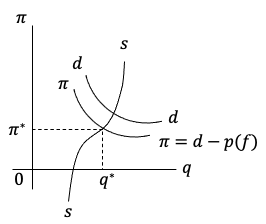
\includegraphics[width=5cm,height=4cm]{EC315-IMG/1.png}
			\item $ss$ = Supply of Crime
			\item $dd$ = Initial Demand
			\item $\pi\pi$ = Demand After Government Intervention ($T$)
			\item $MC$ of Catching Last Criminal $>$ $MB$ [$\leftarrow\pi^*,\ q^*$]
			\item $MC$ of Catching Last Criminal $<$ $MB$ [$\pi^*,\ q^*\rightarrow$]
		\end{itemize}
	\end{enumerate}

	\newpage

	\subsection{Exam Arithmetic Summary}

	\begin{enumerate}
	\setlength\itemsep{0cm}
		\item $\pi_A=x_Ap_A(x_A+x_B)-x_A$
		\item $J=\pi_A+\pi_B;\ \frac{\partial J}{\partial x_A}=\frac{\partial\pi_A}{\partial x_A}+\frac{\partial\pi_B}{\partial x_B}$
		\item Externalities: $\frac{\partial\pi_A}{\partial x_B}$
		\begin{itemize}
			\item $>0$: Positive: ``you do $\uparrow$, my $\pi$ $\uparrow$''
			\item $<0$: Negative: ``you do $\uparrow$, my $\pi$ $\downarrow$''
		\end{itemize}
		\item Strategic Nature: $\frac{\frac{\partial\pi_A}{\partial x_A}}{\partial x_B}$
		\begin{itemize}
			\item $>0$: Complements: ``you do $\uparrow$, I do $\uparrow$''
			\item $<0$: Substitutes: ``you do $\uparrow$, I do $\downarrow$''
		\end{itemize}
		\item Grim Trigger Strategy
		\begin{itemize}
			\item 40, 50, 30
			\item $\frac{40}{(1-\delta)}\ge50+\frac{30\delta}{(1-\delta)}$
			\item $40\ge50-50\delta+30\delta$
			\item $\delta\ge\frac{1}{2}$: cooperation possible
		\end{itemize}
		Tit-for-Tat Strategy
		\begin{itemize}
			\item 40, 50, 20
			\item $\frac{40}{(1-\delta)}\ge\frac{50}{(1-\delta^2)}+\frac{30\delta}{(1-\delta^2)}$
			\item $40+40\delta\ge50+20\delta$
			\item $\delta\ge\frac{1}{2}$: cooperation easy
		\end{itemize}
	\end{enumerate}



















\end{document}
